%%%%%%%%%%%%%%%%%%%%%%%%%%%%%%%%%%%%%%%%%%%%%%%%%%
%%%%%%%%%%%%%%%%%%%%%%%%%%%%%%%%%%%%%%%%%%%%%%%%%%
%%
%% Based one the "beamer-greek-two" template provided 
%% by the Laboratory of Computational Mathematics, 
%% Mathematical Software and Digital Typography, 
%% Department of Mathematics, University of the Aegean
%% (http://myria.math.aegean.gr/labs/dt/)
%%
%% Adapted by John Liaperdos, October-November 2014
%% (ioannis.liaperdos@gmail.com)
%%
%% Last update: 22/06/2017 (English Support)
%%
%%%%%%%%%%%%%%%%%%%%%%%%%%%%%%%%%%%%%%%%%%%%%%%%%%
%%%%%%%%%%%%%%%%%%%%%%%%%%%%%%%%%%%%%%%%%%%%%%%%%%
%%

\documentclass{beamer} 
\usepackage{babel}
\usepackage{caption}
\usepackage{color}
\usepackage{amsmath}
\usepackage{amssymb}

\usepackage{epstopdf}
\usepackage{graphicx}
\usepackage{soul}
\usepackage[utf8]{inputenc}

\usepackage{hyperref}
\usepackage{xstring}
\graphicspath{{./images/}}


\PassOptionsToPackage{unicode}{hyperref}
\PassOptionsToPackage{naturalnames}{hyperref}
\captionsetup[table]{font=scriptsize}

\usepackage{booktabs}

%%
% load TEI-Pel - specific layout
\usepackage{TeiPel_En_Beamer_Layout}
\setTeipelLayout{draft,newlogo}% options: "draft", "newlogo"
\newcommand{\nologo}{\setbeamertemplate{logo}{}} 

%%%%%%%%%%%%%%%%%%%%%%%%%%%%%%%%%%%%%%%%%%%%%%%%%%%%%%%%%%%%
% Thesis Info %%%%%%%%%%%%%%%%%%%%%%%%%%%%%%%%%%%%%%%%%%%%%%
%%%%%%%%%%%%%%%%%%%%%%%%%%%%%%%%%%%%%%%%%%%%%%%%%%%%%%%%%%%%
	% title
		\title{Joint classification of Key-Phrases and Relations in Electronic Health Documents}	
	% author 
    % (In the mandatory argument "{}", separate multiple
    % authors with "\and" - use "\\" for better author name formatting
    % in the title page. In the optional argument "[]" include all
	% author names, with no "\and" or text formatting macros.)
	% Example: 
    %\author[A. Author Albert Einstein]{Anthony Author \and Albert Einstein}
		\author[S. Medina, J. Turmo]{Salvador Medina and Jordi Turmo}
    % Address
   \subtitle{\textsc{Sentiment Analysis at SEPLN (TASS) 2018}}
	\logo{\begin{tabular}{c} \includegraphics[height=0.7cm,keepaspectratio]{\smalllogo} \\ \color{talp_color}\scalebox{1.7}{\insertframenumber/\inserttotalframenumber} \end{tabular}}
	\institute{\textsc{Universitat Politècnica de Catalunya} \\
        Talp Research Center \\
        [5pt]{\includegraphics[height=1.5cm,keepaspectratio]{\fulllogo}} \\
        [5pt]{ Carrer de Jordi Girona, 1-3, 08034 Barcelona \\
         \{smedina, turmo\}@cs.upc.edu\\}
        
        }
	% supervisor	
		% \supervisor{Supervisor}{Jordi Turmo}{Professor}
	% date
		\presentationDate{September 18, 2018}
%%%%%%%%%%%%%%%%


\begin{document}

% typeset front slides

\typesetFrontSlides



%%%%%%%%%%%%%%%%%%%%%%%%%%%%%%%%%%%%%%%%%%%%%%%
%
%   INTRODUCTION
%
%%%%%%%%%%%%%%%%%%%%%%%%%%%%%%%%%%%%%%%%%%%%%%%

\section{Introduction}

\subsection{Highlights}

\begin{frame}{Introduction}
	\framesubtitle{About this project}
	\begin{itemize}
		\item Artificial Neural Network model designed for SEPLN's \textbf{TASS 2018, Task 3}
		    \begin{itemize}
		        \item Sub-Task B: Key-Phrase classification
		        \item Sub-Task C: Identification of binary Relations
		        \item * Excludes Sub-Task A (Key-Phrase Identification)
		    \end{itemize}
	    \item Applied to Spanish \textbf{Electronic Health Documents}
	\end{itemize}
\end{frame}


\begin{frame}{Introduction}
	\framesubtitle{Implementation Highlights}
	\begin{itemize}
		\item Based on Convolutional Neural Networks (\textbf{CNN})
		\item Tokens are encoded using pre-trained word2vec \textbf{word-embeddings}
		\item Considers syntactical features
		\begin{itemize}
		    \item Part Of Speech (\textbf{PoS})
		    \item \textbf{Dependency Tree}
		\end{itemize}
		\item \textbf{Simultaneous optimization} for key-phrase classification and relation extraction
		\item \textbf{Data augmentation} of the training corpus
	\end{itemize}
\end{frame}

\subsection{Motivation}
\begin{frame}{Introduction}
	\framesubtitle{Motivation}
	
	Key-phrase classes are defined by their \textbf{relationships} among them $\rightarrow$ tasks B and C are \textbf{correlated}
	
	\hspace{2em}
	
	\begin{block}{Example}
	A verb is an \emph{Action} key-phrase \underline{if and only if} it relates to another \emph{Action} or \emph{Concept} by either being the \emph{subject} or \emph{target}. Phrases are not key-phrases by themselves but \underline{when they relate to} other phrases.
\end{block}

\end{frame}



%%%%%%%%%%%%%%%%%%%%%%%%%%%%%%%%%%%%%%%%%%%%%%%
%
%   IMPLEMENTATION
%
%%%%%%%%%%%%%%%%%%%%%%%%%%%%%%%%%%%%%%%%%%%%%%%

\section{Implementation}

\subsection{Sequence Encoding}


\begin{frame}{Implementation}
\framesubtitle{Sequence Encoding}

%\begin{block}{Tokenization}
%  Documents are splitted and tokenized using \textbf{FreeLing} with \emph{multi-word},
%\emph{quantity} detection and \emph{Named Entity Classification} (NEC)
%modules disabled
%\end{block}

FreeLing 4.1 for document tokenization and syntactical analysis \footnote{With \emph{multi-word}, \emph{quantity} detection and \emph{Named Entity Classification} modules disabled}
\begin{itemize}
\item \textbf{Word-Embedding}: 300-dimensional vectors, \emph{word2vec} format. We used the pre-trained general-purpose vectors from SBWCE \cite{cardellinoSBWCE}, trained from multiple sources.
\item 1-hot encoding of \textbf{distances} to source and destination key-phrases:
\begin{enumerate}
  \item Absolute \# of tokens between
  \item \# of hops in the dependency tree
\end{enumerate}
\item 1-hot encoding of simplified \textbf{Part-of-Speech tag} (\emph{category} and \emph{type}: 33 options)
\end{itemize}

\end{frame}


\subsection{System Layout}

\begin{frame}{Implementation}
	\framesubtitle{System Layout}
    \begin{figure}[ht]
    \centering
    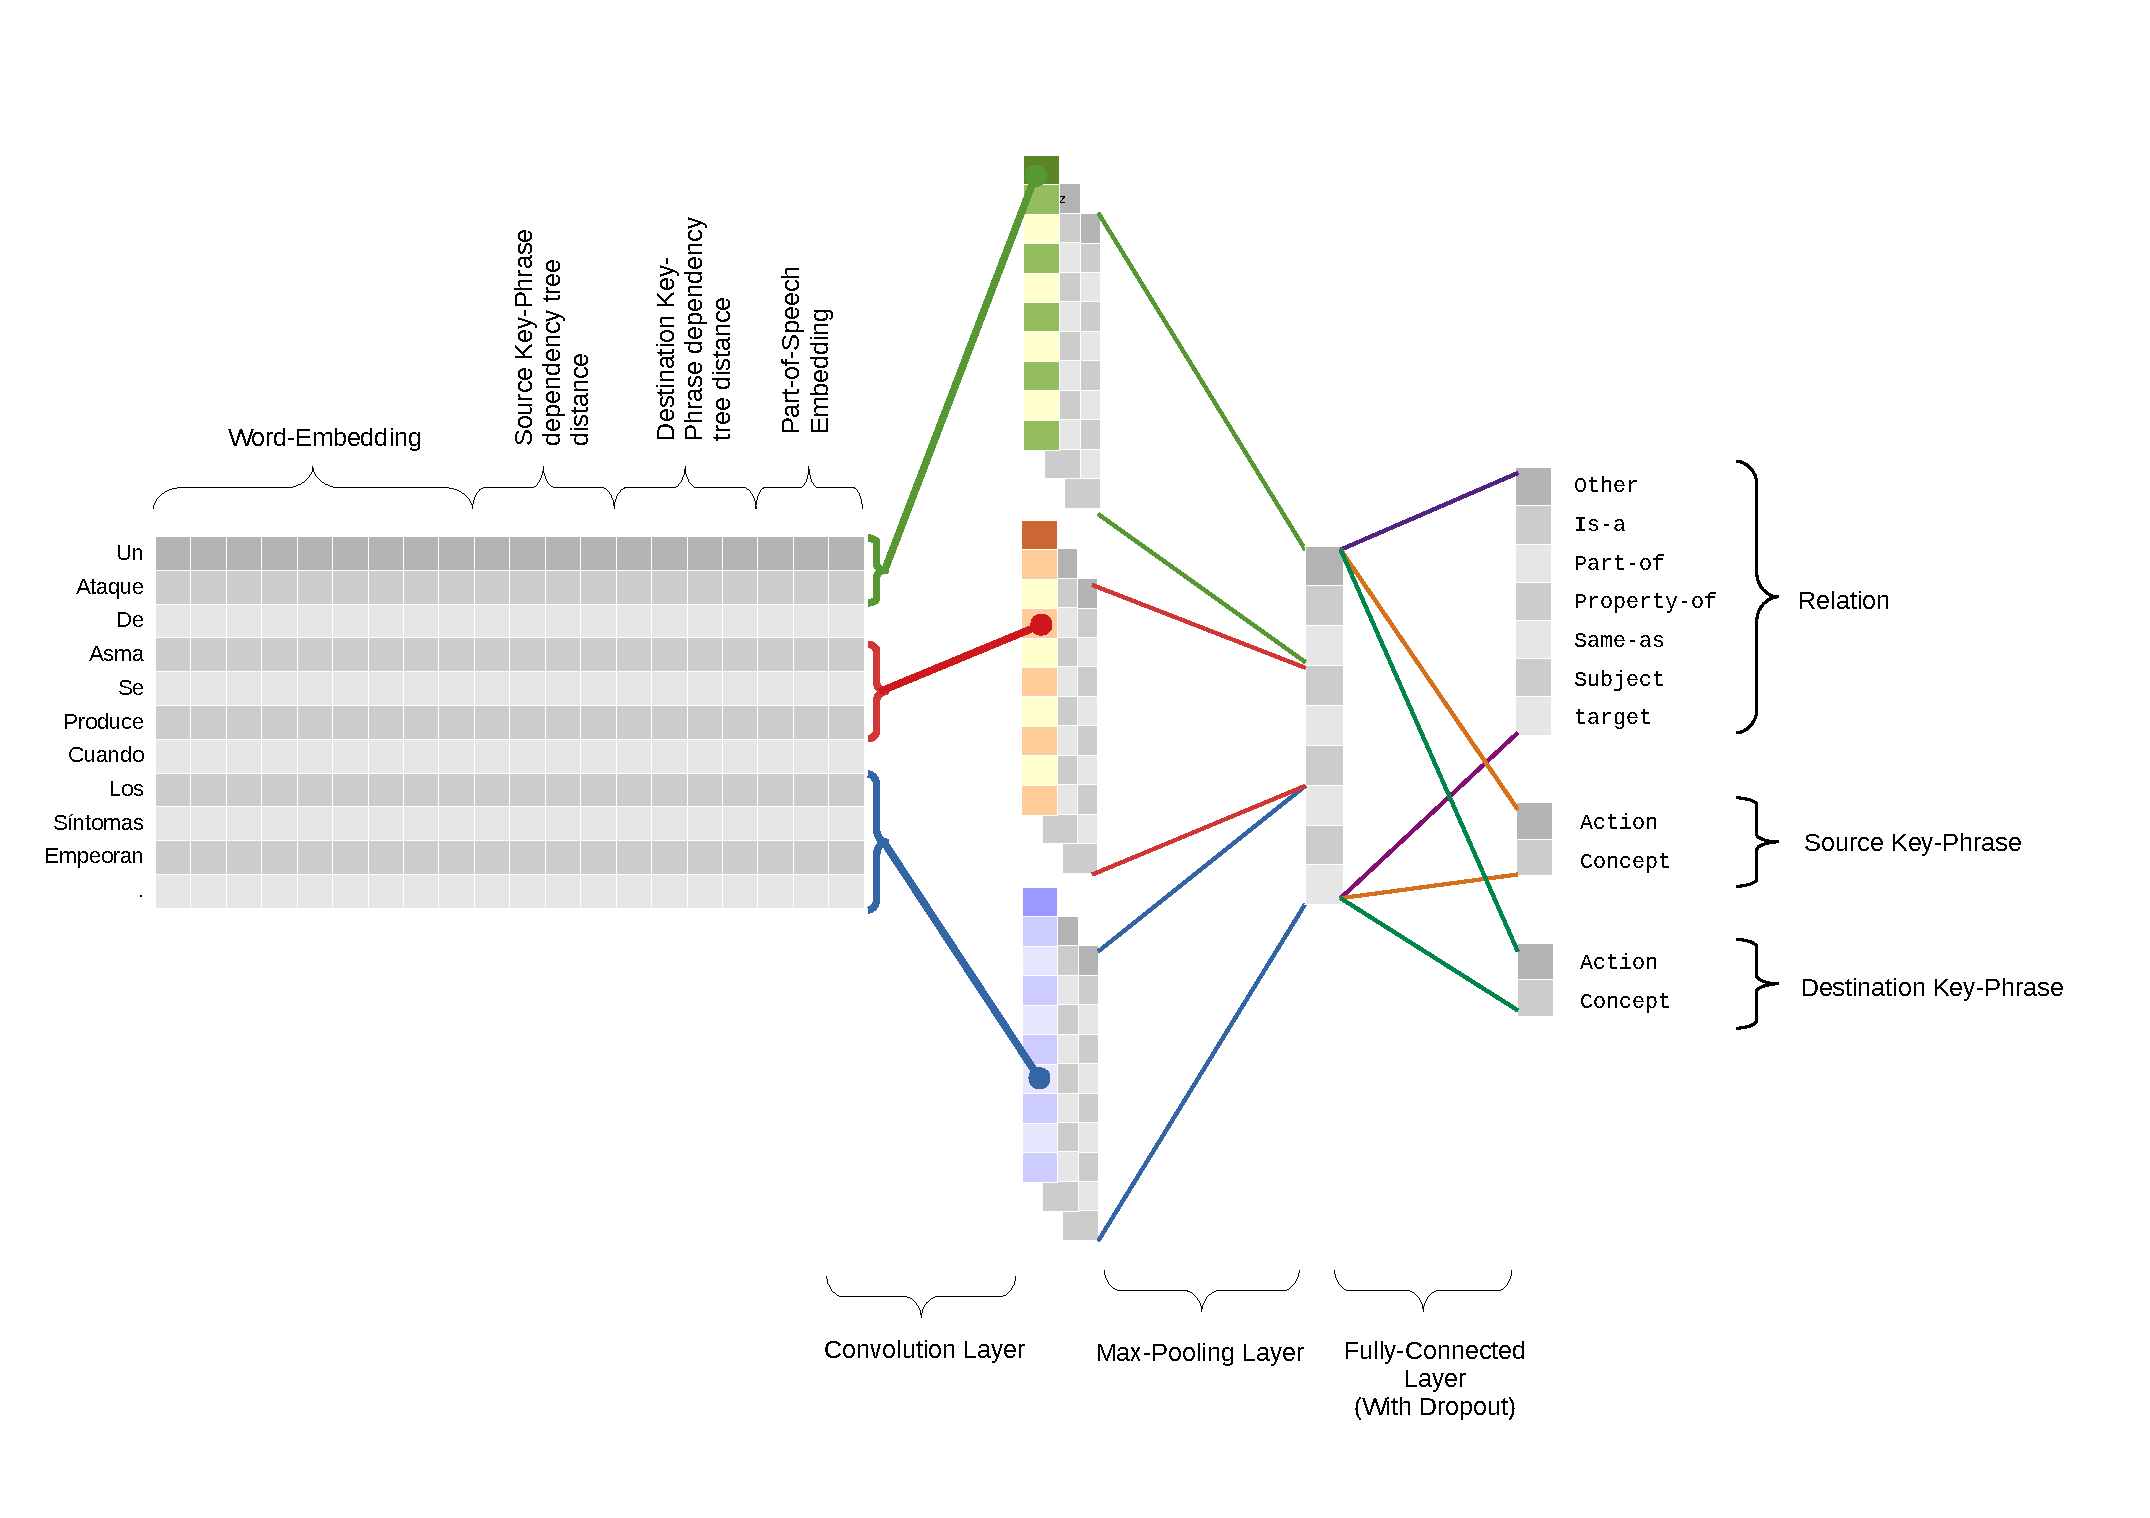
\includegraphics[width=0.9\linewidth,trim={0 1.7cm 0 2.2cm},clip]{diagramtass18.pdf}
    \caption{Layout of the proposed Convolutional Neural Network}
    \label{fig:architecture}
\end{figure}
\end{frame}

\subsection{Parameter Optimization}

\begin{frame}{Implementation}
\framesubtitle{Parameter Optimization}

ANN's weights are optimized for Tasks B and C simultaneously \footnote{CNNs have proven to be capable of jointly identifying entities and relationships in multiple relation extraction tasks \cite{singh2013joint} \cite{shickel2017deep} \cite{li2017neural}}

\begin{itemize}
  \item Independent loss function for each output
  \item Use of \textbf{soft-max cross-entropy}
  \item No relation is encoded with class ``other''
  \item Losses are combined by \textbf{summation}
  \item Parameters are optimized with \emph{TensorFlow's} \emph{Adam} optimizer \footnote{Learning rate of $0.005$. Batches of $128$ documents ($50$ tokens, stripped or padded). Early stopping when the average \emph{loss} in the \emph{development} corpus remains flat for $1000$ iterations}
\end{itemize}

\end{frame}




%%%%%%%%%%%%%%%%%%%%%%%%%%%%%%%%%%%%%%%%%%%%%%%
%
%   RESULTS
%
%%%%%%%%%%%%%%%%%%%%%%%%%%%%%%%%%%%%%%%%%%%%%%%

\section{Results}


\subsection{Overall Results}

\begin{frame}{Results}
\framesubtitle{Overall Results}
    \begin{table}[ht]
    \footnotesize
    \centering
\begin{tabular}{r|cccccc|c}
\toprule
% \rotatebox{90}{Scenario} & \rotatebox{90}{plubeda} & \rotatebox{90}{rriveraz} & \rotatebox{90}{upf\_upc} & \rotatebox{90}{TALP} & \rotatebox{90}{VSP} & \rotatebox{90}{baseline} & \rotatebox{90}{Marcelo} \\
{\footnotesize{scenario}} & {\footnotesize{plubeda}} & {\footnotesize{rriveraz}} & {\footnotesize{upf\_upc}} & {\footnotesize{VSP}} & {\footnotesize{baseline}} & {\footnotesize{Marcelo}} & {\footnotesize{TALP}} \\
\midrule
1 & .71 & \textbf{.744} & .681 & .297 & .566 & .181 & {\footnotesize{N/A*}} \\
2 & .674 & .648 & .622 & .275 & .577 & .255 & \textbf{.722} \\
3 & {\scriptsize{N/A*}} & {\scriptsize{N/A*}} & .036 & .420 & .107 & .018 & \textbf{.448} \\
\bottomrule
avg & .461 & \textbf{.464} & .446 & .331 & .417 & .151 & .39 \\
\end{tabular}
    \caption{Micro-averaged $F1$ score for evaluation scenarios 1 to 3 and global average. \emph{TALP} column shows our model's score. \textbf{N/A*}: Not Available, counted as 0 in the average score.}
    \label{tab:results}
\end{table}
\end{frame}

\subsection{Sub-Task B: Key-Phrase Classification}

\begin{frame}{Results}
\framesubtitle{Sub-Task B: Key-Phrase Classification}
    \begin{table}[t]
 \footnotesize
    \centering
\begin{tabular}{r|cc|c}
\toprule
true\textbackslash pred. & Concept &  Action & recall \\
\midrule
Concept &  \textbf{432} &       7 &  .984\\
Action  &   34 &     \textbf{120} & .779\\
\bottomrule
precision & .927 & .945 & $Acc=.931$


\end{tabular}
    \caption{Confusion matrix of our model's predictions for sub-task \emph{B} in scenario 2.}
    \label{tab:confusion2a}
\end{table}
\end{frame}


\subsection{Sub-Task C: Relation Extraction}

\begin{frame}{Results}
\framesubtitle{Sub-Task C: Relation Extraction}
    \begin{table}[ht]
\footnotesize
    \centering
    \begin{tabular}{r|ccccccc|c}
\toprule
 true\textbackslash pred. &  \rotatebox{90}{other} &  \rotatebox{90}{is-a} &  \rotatebox{90}{part-of} &  \rotatebox{90}{property-of} &  \rotatebox{90}{same-as} &  \rotatebox{90}{subject} &  \rotatebox{90}{target} & \rotatebox{90}{recall}\\
\midrule
other       &      \textbf{0} &     0 &        0 &            0 &        0 &        0 &       0 & .000 \\
is-a        &     31 &    \textbf{58} &        1 &            2 &        0 &        0 &       0 & .630 \\
part-of     &     26 &     2 &        \textbf{5} &            0 &        0 &        0 &       0 & .152 \\
property-of &     34 &     0 &        3 &           \textbf{18} &        0 &        0 &       3 & .310 \\
same-as     &      0 &     1 &        0 &            0 &        \textbf{0} &        0 &       0 & .000 \\
subject     &     65 &     0 &        0 &            2 &        0 &       \textbf{42} &       8 & .359 \\
target      &     84 &     0 &        1 &            7 &        0 &       12 &      \textbf{91} & .467 \\
\bottomrule
precision & .000 & .951 & .500 & .621 & .000 & .778 & .892 & $F_1$=.431
\end{tabular}
    \caption{Confusion matrix, precision and recall of our model's predictions for sub-task \emph{C} in scenario 2. $F_1$ is micro-averaged for all classes.}
    \label{tab:confusion2b}
\end{table}
    
\end{frame}


\subsection{Analysis of Errors}

\begin{frame}{Results}
\framesubtitle{Analysis of Errors I}
\begin{itemize}
  \item Actions are a particular kind of Concept
  
  \begin{itemize}
    \item \footnotesize Concept: ``El
tratamiento depende de la \underline{causa}.'' (The
treatment depends on the \underline{cause}.).
    \item Action: ``Es una \underline{causa} común
de sordera.'' (It is a common \underline{cause} of
deafness.)
% as it modifies ``sordera'' (deafness).
  \end{itemize}

  \item Entites that do not apparently match any labeling criteria
  \begin{itemize}
    \item \footnotesize Action?: ``Si usted ya tiene diabetes, el mejor momento para controlar su diabetes es \underline{antes} de quedar embarazada.'' (If you already have diabetes, the best moment to control your diabetes is \underline{before} getting pregnant.)
  \end{itemize}
  \item Sentence analysis errors (FreeLing)
  \begin{itemize}
    \item \footnotesize $noun \rightarrow verb$: ``Suele afectar s\'{o}lo un \underline{o\'{i}do}.'' (It usually affects just one \underline{ear}.)
    \item $verb \rightarrow noun$: ``Esto \underline{causa} una acumulaci\'{o}n de sustancias grasosas en el bazo, h\'{i}gado, pulmones, huesos y, a veces, en el cerebro.'' (This \underline{causes} an accumulation of fatty substances in the arm, liver, lungs, bones and sometimes, the brain.)
  \end{itemize}
\end{itemize}
\end{frame}


\begin{frame}{Results}
\framesubtitle{Analysis of Errors II}
\begin{itemize}
    \item Corpus is strongly unbalanced: Much lower \emph{recall} and \emph{precision} in uncommon classes: \emph{same-as}, \emph{part-of}, ...
      \item Confusion between \emph{subject} and \emph{target} (Reflexiveness)
      \begin{itemize}
        \item \footnotesize Subject: ``\emph{Algunos \underline{sarpullidos} \underline{se desarrollan} inmediatamente.}'' (Some \underline{skin rashes} \underline{are developed} immediately.)
        \item Target: ``\emph{\underline{Existen} muchas \underline{razones} para someterse a una cirug\'{i}a.}'' (\underline{There are} several \underline{reasons} to have surgery.)
      \end{itemize}
      \item Multi-label relationship was not considered by our model
\end{itemize}
\end{frame}


%%%%%%%%%%%%%%%%%%%%%%%%%%%%%%%%%%%%%%%%%%%%%%%
%
%   CONCLUSIONS & FUTURE WORK
%
%%%%%%%%%%%%%%%%%%%%%%%%%%%%%%%%%%%%%%%%%%%%%%%

\section{Final Remarks}

\subsection{Conclusions}

\begin{frame}{Final Remarks}
\framesubtitle{Summary}

\begin{itemize}
  \item The results prove that joint classification outperforms traditional two-step methods
  \item \textbf{Correlation} between \emph{key-phrase classes} and \emph{relation classes} can be exploited
  \item Relation extraction is \textbf{hard}
  \begin{itemize}
    \item Available corpora is small
    \item Relations are often ambiguous
    \item Dependency parsing and PoS is not perfect
  \end{itemize}
\end{itemize}
\end{frame}

\subsection{Future Work}

\begin{frame}{Final Remarks}
\framesubtitle{Future Work}

\begin{itemize}
  \item Deal with \textbf{multi-label} relationships
  \item Make use of the \textbf{full morphosyntactic} analysis
  \item Use of more aggressive \textbf{regularization} and \textbf{data augmentation} techniques
  \item Identify \textbf{key-phrase's boundaries} \footnote{We already have a working prototype using Convolutional and Recurrent Neural Networks for joint NERC and Relation extraction.}
  \item Define \textbf{specific optimization} functions (loss) for joint classification scenarios
\end{itemize}

\end{frame}


\section*{Acknowledgements and References}

%%%%%%%%%%%%%%%%%%%%%%%%%%%%%%%%%%%%%%%%%%%%%%%
%
%   CLOSING
%
%%%%%%%%%%%%%%%%%%%%%%%%%%%%%%%%%%%%%%%%%%%%%%%

\begin{frame}{Acknowledgements}
  \centering
This works has been partially funded by the Spanish Government and by the European Union through GRAPHMED project (TIN2016-77820-C3-3-R and AEI/FEDER,UE.)

\end{frame}

\begin{frame}[allowframebreaks]{References}
\bibliographystyle{apalike}
\bibliography{bibliography.bib}
\end{frame}

\begin{frame}
\centering
\Huge Thank you for your attention!
\Huge Questions?
\end{frame}



%%
\end{document}
